\documentclass[10pt]{article}
\usepackage[letterpaper,margin=1in]{geometry}
\usepackage[T1]{fontenc}
\usepackage{lmodern}
\usepackage{amsmath,amssymb}
\usepackage{graphicx}
\usepackage{booktabs}
\usepackage{xcolor}
\usepackage[numbers,sort&compress]{natbib}
\usepackage{tikz}
\usepackage[colorlinks=true,linkcolor=blue!50!black,citecolor=blue!50!black,urlcolor=blue!50!black]{hyperref}
\usetikzlibrary{positioning}
\newcommand{\TODO}[1]{\textcolor{red}{\textbf{[TODO: #1]}}}
\newcommand{\ket}[1]{\lvert #1\rangle}
% Generated by figures_scripts/make_values.py; do not edit.
\newcommand{\valCeilThree}{0.840}
\newcommand{\valNTrainFullThree}{11{,}922}
\newcommand{\valPatternsThree}{44}
\newcommand{\valCeilFour}{0.916}
\newcommand{\valNTrainFullFour}{11{,}520}
\newcommand{\valPatternsFour}{193}
\newcommand{\valNTestFull}{1{,}968}
\newcommand{\valQnnAcc}{0.868}
\newcommand{\valQnnStd}{0.023}
\newcommand{\valQnnParams}{32}
\newcommand{\valQnnSecs}{543}
\newcommand{\valHybridAcc}{0.906}
\newcommand{\valHybridStd}{0.006}
\newcommand{\valHybridParams}{185}
\newcommand{\valHybridSecs}{636}
\newcommand{\valClassicalAcc}{0.909}
\newcommand{\valClassicalStd}{0.006}
\newcommand{\valClassicalParams}{37}
\newcommand{\valClassicalSecs}{5}
\newcommand{\valMnistNTrain}{3000}
\newcommand{\valMnistNTest}{500}
\newcommand{\valMnistEpochs}{4}
\newcommand{\valMnistSeeds}{3}
\newcommand{\valMnistBatch}{32}
\newcommand{\valMnistLr}{0.01}
\newcommand{\valHybridGain}{3.8}
\newcommand{\valBpDecay}{0.71}
\newcommand{\valBpCircuits}{200}
\newcommand{\valBpFixedDepth}{50}
\newcommand{\valBpFixedQubits}{8}
\newcommand{\valBpMinQ}{2}
\newcommand{\valBpMaxQ}{12}
\newcommand{\valBpVarMinQ}{$8.6\times10^{-2}$}
\newcommand{\valBpVarMaxQ}{$2.8\times10^{-3}$}
\newcommand{\valBpRatio}{31}
\newcommand{\valBpRatioEight}{27}
\newcommand{\valBpVarEight}{$3.2\times10^{-3}$}
\newcommand{\valBpDepthRatio}{38}
\newcommand{\valBpMinDepth}{1}
\newcommand{\valBpMaxDepth}{50}
\newcommand{\valBpVarShallow}{$9.9\times10^{-2}$}
\newcommand{\valBpVarDeep}{$2.6\times10^{-3}$}
\newcommand{\valNoiseSize}{3}
\newcommand{\valNoiseQubits}{10}
\newcommand{\valNoiseNTrain}{200}
\newcommand{\valNoiseNTest}{200}
\newcommand{\valNoiseEvalNTest}{500}
\newcommand{\valNoiseBatch}{16}
\newcommand{\valNoiseLr}{0.02}
\newcommand{\valNoiseEpochs}{3}
\newcommand{\valNoiseReps}{50}
\newcommand{\valNoiseSeeds}{3}
\newcommand{\valNoiseMaxP}{0.03}
\newcommand{\valNoiseTrClean}{0.862}
\newcommand{\valNoiseTrMax}{0.753}
\newcommand{\valNoiseEvClean}{0.859}
\newcommand{\valNoiseEvMax}{0.501}
\newcommand{\valNoiseEvMid}{0.770}
\newcommand{\valNoiseTrMid}{0.859}
\newcommand{\valVerTF}{2.18.1}
\newcommand{\valVerTFQ}{0.7.6}
\newcommand{\valVerCirq}{1.5.0}

\typeout{PROBE textwidth=\the\textwidth}

\title{Training Quantum Neural Networks with TensorFlow Quantum:\\a Small, Reproducible Study}
\author{\TODO{author name(s) and affiliation}}
\date{}

\begin{document}
\maketitle
\begin{abstract}
Quantum neural networks (QNNs) are easy to describe and surprisingly hard to evaluate fairly. We
present a small, fully reproducible study built on TensorFlow Quantum, aimed at readers who want to see
the main behaviours of QNN training first-hand. A 17-qubit Farhi--Neven QNN learns to separate 3s from
6s in $4\times4$ binarised MNIST, reaching \valQnnAcc{} test accuracy over \valMnistSeeds{} seeds. A
classical network with \valClassicalParams{} weights reaches \valClassicalAcc{}, and adding an 8-unit
classical head to the same circuit lifts it to \valHybridAcc{}. Both are close to the \valCeilFour{}
that a lookup table over the training patterns sets as a ceiling for this input. Gradient variance in
random circuits falls \valBpRatioEight-fold from 2 to 8 qubits. Under depolarizing noise, models
trained without noise drop to \valNoiseEvMid{} at $p=0.01$ and to chance at $p=\valNoiseMaxP$. Code,
raw results and the scripts that generate every number in this paper are released.
\end{abstract}

\section{Introduction}
\label{sec:intro}

Parameterised quantum circuits trained by gradient descent are the most common model in near-term
quantum machine learning \citep{preskill2018nisq,cerezo2021vqa}. Software such as TensorFlow Quantum
(TFQ) \citep{broughton2020tfq} lets anyone train them on a laptop. That makes it easy to run a demo, and
also easy to misread one: without a matched classical baseline, a sense of what the data allows, or a
look at gradients and noise, a working QNN says little.

This paper is a compact, reproducible tour of those checks on one task: the Farhi--Neven QNN
\citep{farhi2018classification} on $4\times4$ MNIST 3-vs-6, the setting of the TFQ tutorial. We contribute:
\begin{itemize}
  \item a matched comparison of the QNN, a classical network of similar size, and a hybrid model that
        adds a classical head to the same circuit, alongside the accuracy ceiling the input allows
        (\S\ref{sec:res-mnist}, \S\ref{sec:res-hybrid});
  \item measurements of gradient variance in random circuits as width and depth grow
        (\S\ref{sec:res-barren});
  \item the effect of depolarizing noise, both on trained models and during training
        (\S\ref{sec:res-noise});
  \item code that regenerates every figure, table and number from raw results with one command,
        running on current TFQ (\valVerTFQ) in Docker.
\end{itemize}
None of these phenomena are new. The point is to reproduce them together, with error bars, in a form
that is easy to rerun and extend.

\section{Background}
\label{sec:background}

\paragraph{Quantum neural networks.}
A parameterised quantum circuit (PQC) applies gates whose angles are trainable, and its output is the
expectation value of an observable. Trained by gradient descent, PQCs are the near-term analogue of neural
networks \citep{preskill2018nisq,cerezo2021vqa}. \citet{farhi2018classification} proposed a QNN for binary
classification in which every data qubit couples to a single readout qubit, and the prediction is
$\langle Z\rangle$ on that readout. We use their architecture throughout.

\paragraph{Gradients.}
On hardware, gradients come from the parameter-shift rule, which evaluates the circuit at shifted
angles \citep{mitarai2018qcl,schuld2019gradients}. In exact classical simulation, the adjoint method gives
all gradients at roughly the cost of one forward and one backward pass \citep{jones2020adjoint}.

\paragraph{Barren plateaus.}
For sufficiently random circuits, the variance of the gradient with respect to any parameter decays
exponentially in the number of qubits \citep{mcclean2018barren}. Hardware noise can induce the same
effect even in shallow circuits \citep{wang2021noise}.

\paragraph{TensorFlow Quantum.}
TFQ \citep{broughton2020tfq} represents circuits (built with Cirq) as tensors and exposes simulation,
expectation values and their gradients as Keras layers on top of TensorFlow \citep{abadi2016tensorflow}.
The same model code can use exact, noisy or sampled simulation. Its tutorials include a version of the
Farhi--Neven MNIST task, which we follow for the data pipeline. \citet{huang2021power} discuss when
classical models can match quantum ones on data like this, which is relevant to our baseline.

\section{Setup}
\label{sec:setup}

\paragraph{Data.}
We keep the 3s and 6s from MNIST \citep{lecun1998mnist} and downsample each image to $4\times4$ by
bilinear resizing. As in the TFQ tutorial, we then remove training images whose downsampled form occurs
with both labels, and binarise every pixel at a threshold of 0.5. Each lit pixel becomes an $X$ gate,
so an image is the basis state $\ket{x}$ of 16 data qubits. Each seed draws \valMnistNTrain{} training
and \valMnistNTest{} test images at random.

\paragraph{Models.}
\emph{QNN.} A readout qubit is prepared with $X$ then $H$. Every data qubit $i$ then couples to it
through $XX^{\theta_i}$, then $ZZ^{\phi_i}$, and a final $H$ is applied to the readout
(Fig.~\ref{fig:circuit}). The prediction is $\langle Z\rangle\in[-1,1]$ on the readout, giving
\valQnnParams{} parameters on 17 qubits. \emph{Hybrid.} The same circuit, but $\langle Z\rangle$ on all
17 qubits feeds a dense layer with 8 ReLU units and a $\tanh$ output (\valHybridParams{} parameters).
\emph{Classical.} A multilayer perceptron on the same 16 binary pixels, with 2 ReLU units and a $\tanh$
output (\valClassicalParams{} parameters), chosen to roughly match the QNN's parameter count.

\begin{figure}[t]
\centering
% Schematic of the Farhi--Neven QNN (hand-drawn TikZ, no data).
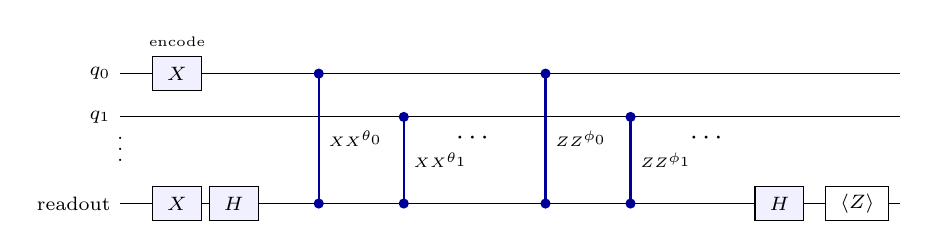
\begin{tikzpicture}[x=0.9cm,y=0.55cm,
  g/.style={draw,fill=blue!6,minimum width=0.62cm,minimum height=0.44cm,inner sep=1pt,font=\scriptsize},
  dot/.style={circle,fill=blue!60!black,inner sep=1.3pt}]
  \foreach \y/\n in {2/{$q_0$},1/{$q_1$}} \draw (0,\y) node[left,font=\scriptsize]{\n} -- (11,\y);
  \node[font=\scriptsize] at (0,0.45) {$\vdots$};
  \draw (0,-1) node[left,font=\scriptsize]{readout} -- (11,-1);
  \node[g] at (0.8,2) {$X$};
  \node[font=\tiny,above] at (0.8,2.4) {encode};
  \node[g] at (0.8,-1) {$X$}; \node[g] at (1.6,-1) {$H$};
  \foreach \x/\y/\l in {2.8/2/XX^{\theta_0},4.0/1/XX^{\theta_1},6.0/2/ZZ^{\phi_0},7.2/1/ZZ^{\phi_1}} {
    \draw[blue!60!black,thick] (\x,\y) -- (\x,-1);
    \node[dot] at (\x,\y) {}; \node[dot] at (\x,-1) {};
    \node[font=\tiny,right] at (\x,{(\y-1)/2}) {$\l$};
  }
  \node at (5.0,0.5) {$\cdots$}; \node at (8.3,0.5) {$\cdots$};
  \node[g] at (9.3,-1) {$H$};
  \node[g,fill=white,minimum width=0.8cm] at (10.4,-1) {$\langle Z\rangle$};
\end{tikzpicture}

\caption{The QNN circuit, with two of the 16 data qubits drawn. Each data qubit couples to the
readout qubit through one trainable $XX$ gate and one trainable $ZZ$ gate.}
\label{fig:circuit}
\end{figure}

\paragraph{Training.}
All models minimise the hinge loss on labels $\pm1$ with Adam \citep{kingma2014adam} (learning rate
\valMnistLr{}, batch size \valMnistBatch{}) for \valMnistEpochs{} epochs, over \valMnistSeeds{} seeds.
Quantum models are simulated exactly and differentiated with the adjoint method. We report mean
$\pm$ standard deviation over seeds. We chose the batch size and learning rate from two candidate
settings on seed 0.

\paragraph{Barren plateaus.}
Following \citet{mcclean2018barren}, each random circuit applies $R_y(\pi/4)$ to every qubit, then
layers of a uniformly random choice of $R_x$, $R_y$ or $R_z$ per qubit followed by a CZ ladder. We
estimate $\mathrm{Var}[\partial\langle Z_0Z_1\rangle/\partial\theta_0]$ over \valBpCircuits{} random
circuits and angles, sweeping \valBpMinQ--\valBpMaxQ{} qubits at \valBpFixedDepth{} layers, and
\valBpMinDepth--\valBpMaxDepth{} layers at \valBpFixedQubits{} qubits.

\paragraph{Noise.}
A single-qubit depolarizing channel with probability $p$ follows every moment of the model circuit.
Expectations average \valNoiseReps{} quantum trajectories. We run two measurements. (i) The
$4\times4$ QNNs trained above are tested under noise on \valNoiseEvalNTest{} test images (a separate
random draw from the one in Table~\ref{tab:mnist}, so the noise-free accuracies differ slightly). (ii) Models
are trained and tested with the noise present. Training through trajectories needs parameter-shift
gradients, which made 17 qubits too slow, so (ii) uses $\valNoiseSize\times\valNoiseSize$ images
(\valNoiseQubits{} qubits), \valNoiseNTrain{} training and \valNoiseNTest{} test images,
\valNoiseEpochs{} epochs, batch size \valNoiseBatch{} and learning rate \valNoiseLr{}.

\paragraph{Software and hardware.}
TensorFlow \valVerTF, TensorFlow Quantum \valVerTFQ{} and Cirq \valVerCirq, in a Linux Docker container
with 8 CPU cores on an Intel laptop, with no GPU.

\section{Results}
\label{sec:results}

\subsection{The QNN learns the task, and a classical network of similar size does slightly better}
\label{sec:res-mnist}

\begin{table}[t]
\centering
\caption{Test accuracy on $4\times4$ binarised MNIST 3-vs-6 (mean $\pm$ std over \valMnistSeeds{} seeds,
\valMnistNTrain{} training and \valMnistNTest{} test images per seed, \valMnistEpochs{} epochs). A
lookup table over training patterns reaches \valCeilFour{}. Training time is the mean wall-clock time
of simulated training on CPU. It varied by up to $3\times$ across seeds with machine load.}
\label{tab:mnist}
\begin{tabular}{lrrr}
\toprule
Model & Parameters & Test accuracy & Train time (s) \\
\midrule
QNN (quantum readout) & 32 & 0.868 $\pm$ 0.023 & 543 \\
QNN + dense head (hybrid) & 185 & 0.906 $\pm$ 0.006 & 636 \\
classical MLP & 37 & \textbf{0.909 $\pm$ 0.006} & 5 \\
\bottomrule
\end{tabular}

\end{table}

\begin{figure}[t]
\centering
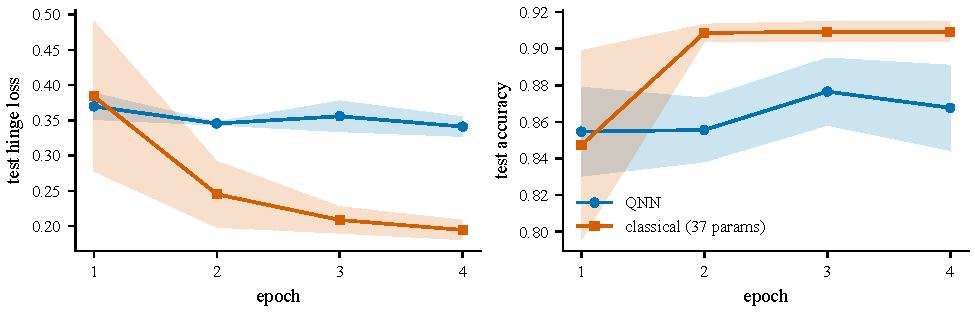
\includegraphics[width=\linewidth]{figures/mnist_qnn.pdf}
\caption{The classical network overtakes the QNN after the first epoch and ends higher, with less spread across seeds.
Test hinge loss and accuracy per epoch, mean $\pm$ std over \valMnistSeeds{} seeds.}
\label{fig:mnist}
\end{figure}

The QNN reaches \valQnnAcc{} $\pm$ \valQnnStd{} test accuracy (Table~\ref{tab:mnist},
Fig.~\ref{fig:mnist}). The classical network, with \valClassicalParams{} parameters against the QNN's
\valQnnParams{}, reaches \valClassicalAcc{} $\pm$ \valClassicalStd{}. Both are bounded by the input:
binarising to $4\times4$ leaves \valPatternsFour{} distinct training patterns, and predicting each
pattern's majority label scores \valCeilFour{} on the full test set. The classical model sits almost on
that ceiling, so on this input there is little room for any model to do better. The QNN also took about
\valQnnSecs{}\,s to train in simulation, against \valClassicalSecs{}\,s for the classical network.

\subsection{A classical head on the readouts closes the gap}
\label{sec:res-hybrid}

\begin{figure}[t]
\centering
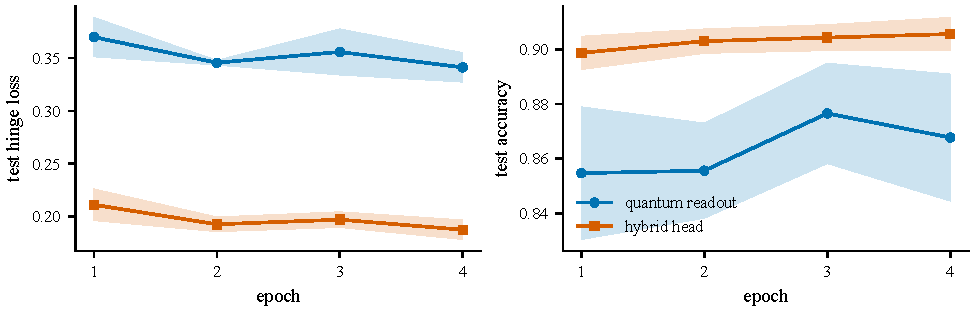
\includegraphics[width=\linewidth]{figures/hybrid.pdf}
\caption{Reading out every qubit and adding a small dense head improves accuracy and reduces
variance across seeds. Same data, seeds and circuit as Fig.~\ref{fig:mnist}.}
\label{fig:hybrid}
\end{figure}

Measuring $\langle Z\rangle$ on all 17 qubits and passing the values through an 8-unit dense layer raises
accuracy by \valHybridGain{} points, to \valHybridAcc{} $\pm$ \valHybridStd{} (Fig.~\ref{fig:hybrid}).
This matches the classical model. The gain cannot be attributed to the circuit alone: the hybrid model
has \valHybridParams{} parameters, most of them classical, and 16 of its 17 readouts are on data qubits, which
start in the input's basis state.

\subsection{Gradients shrink as random circuits grow}
\label{sec:res-barren}

\begin{figure}[t]
\centering
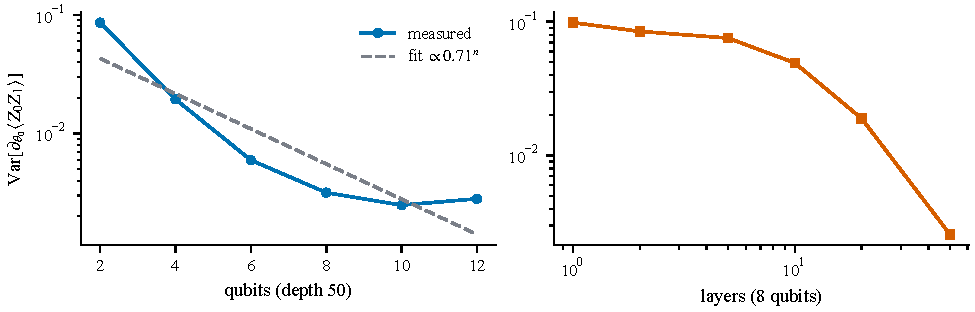
\includegraphics[width=\linewidth]{figures/barren_plateaus.pdf}
\caption{Gradient variance falls with width and with depth. Left: variance of
$\partial\langle Z_0Z_1\rangle/\partial\theta_0$ against qubit count at \valBpFixedDepth{} layers, with a
log-linear fit over all points. Right: against depth at \valBpFixedQubits{} qubits. Each point uses
\valBpCircuits{} random circuits.}
\label{fig:barren}
\end{figure}

At \valBpFixedDepth{} layers, the gradient variance falls from \valBpVarMinQ{} at \valBpMinQ{} qubits to
\valBpVarEight{} at 8 qubits, a factor of \valBpRatioEight{} (Fig.~\ref{fig:barren}, left). Beyond 8
qubits it stops falling in our sweep, reaching \valBpVarMaxQ{} at \valBpMaxQ{} qubits, so a single
exponential (decay factor \valBpDecay{} per qubit) describes the trend only loosely. The depth sweep
suggests why. At \valBpFixedQubits{} qubits the variance is still falling at \valBpMaxDepth{} layers,
\valBpDepthRatio{} times below its single-layer value (Fig.~\ref{fig:barren}, right), so
\valBpFixedDepth{} layers are probably not enough for the wider circuits to behave as random as the
theory assumes \citep{mcclean2018barren}. We did not test this directly.

\subsection{Depolarizing noise erodes accuracy quickly}
\label{sec:res-noise}

\begin{figure}[t]
\centering
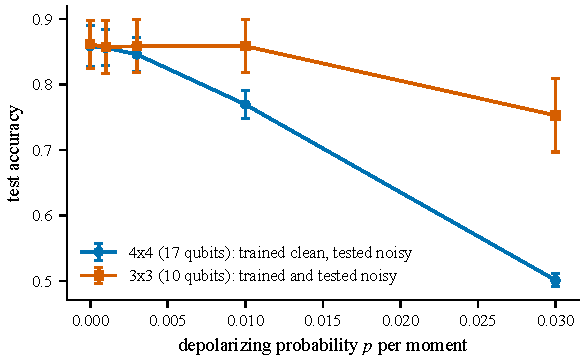
\includegraphics[width=0.6\linewidth]{figures/noise.pdf}
\caption{Trained $4\times4$ QNNs fall to chance by $p=\valNoiseMaxP$. Smaller $3\times3$ models
trained with the noise present hold their accuracy up to $p=0.01$. The two curves are different
models with different circuit depths, so compare slopes, not heights. Mean $\pm$ std over
\valNoiseSeeds{} seeds; \valNoiseReps{} trajectories per expectation.}
\label{fig:noise}
\end{figure}

\begin{table}[t]
\centering
\caption{Test accuracy under depolarizing noise with probability $p$ per qubit per moment (mean $\pm$ std over
\valNoiseSeeds{} seeds).}
\label{tab:noise}
\begin{tabular}{lcc}
\toprule
$p$ & 3$\times$3, trained with noise & 4$\times$4, trained clean, tested with noise \\
\midrule
0.0 & 0.862 $\pm$ 0.036 & 0.859 $\pm$ 0.031 \\
0.001 & 0.857 $\pm$ 0.040 & 0.856 $\pm$ 0.028 \\
0.003 & 0.859 $\pm$ 0.040 & 0.846 $\pm$ 0.026 \\
0.01 & 0.859 $\pm$ 0.040 & 0.770 $\pm$ 0.022 \\
0.03 & 0.753 $\pm$ 0.056 & 0.501 $\pm$ 0.010 \\
\bottomrule
\end{tabular}

\end{table}

The $4\times4$ QNNs from \S\ref{sec:res-mnist}, tested under noise, go from \valNoiseEvClean{} without
noise to \valNoiseEvMid{} at $p=0.01$ and \valNoiseEvMax{} at $p=\valNoiseMaxP$, which is chance
(Fig.~\ref{fig:noise}, Table~\ref{tab:noise}). The channel acts after every moment of a circuit with 32
two-qubit couplings, so errors accumulate before the readout is measured. The $3\times3$ models trained with the noise
present keep \valNoiseTrMid{} at $p=0.01$, against \valNoiseTrClean{} without noise, and drop to
\valNoiseTrMax{} at $p=\valNoiseMaxP$. This comparison is confounded: the $3\times3$ circuit has 18
couplings rather than 32, so it accumulates less noise whether or not it is trained with it. Separating
the effect of noise-aware training from circuit size would need noisy training at $4\times4$, which was
too slow for us (\S\ref{sec:setup}).

\section{Limitations}
\label{sec:limitations}

Everything here is classical simulation of small circuits. The task (two digits at $4\times4$ binary
pixels) is far from where a quantum advantage could appear, and the input is so coarse that even a
lookup table over training patterns sets a ceiling well below standard MNIST accuracies. We ran
\valMnistSeeds{} seeds and lightly tuned two hyperparameters on one seed, so small differences
between models should not be over-read. The noisy-training study uses smaller $3\times3$ images than the
rest of the paper, and every noisy expectation carries trajectory-sampling error on top of the channel
itself. The barren-plateau sweep stops at \valBpMaxQ{} qubits, with \valBpCircuits{} circuits per point.
None of these results are new. They reproduce known behaviour with current open-source tools.

\section{Conclusion}
\label{sec:conclusion}

TensorFlow Quantum makes the full loop (encoding classical data as circuits, training a QNN as a Keras
layer, switching to noisy simulation, and probing gradient statistics) a few hundred lines of Python
that run on a laptop CPU. On this small task, a classical model of similar size matches or beats the QNN, a
classical head on the circuit's readouts brings the QNN up to that baseline, gradient variance shrinks as
random circuits grow, and depolarizing noise quickly erodes a trained model's accuracy. These are the behaviours a newcomer to quantum machine
learning should expect to see.

\paragraph{Reproducibility.}
All code, configurations and raw results ship with this paper. One command
(\texttt{python -m quantumtf\_demo.run\_all -{}-preset full}) reruns every experiment in Docker. Every
number in the text is generated from the result files by a script, and \texttt{sources.md} records where
each value comes from.

\label{pw:mainend}
\section*{Use of AI tools}
An AI assistant (Claude) wrote the experiment code, ran the experiments, generated the figure and
table scripts, drafted the text and checked the references against arXiv and Crossref. The
author chose the scope and the experiments.

\bibliographystyle{plainnat}
\bibliography{refs}
\end{document}
